\documentclass[12pt, titlepage]{article}

\usepackage{fullpage}
\usepackage[round]{natbib}
\usepackage{multirow}
\usepackage{booktabs}
\usepackage{tabularx}
\usepackage{graphicx}
\usepackage{float}
\usepackage{hyperref}
\usepackage{enumerate}
\hypersetup{
    colorlinks,
    citecolor=blue,
    filecolor=black,
    linkcolor=red,
    urlcolor=blue
}

%% Comments

\usepackage{color}

\newif\ifcomments\commentstrue %displays comments
%\newif\ifcomments\commentsfalse %so that comments do not display

\ifcomments
\newcommand{\authornote}[3]{\textcolor{#1}{[#3 ---#2]}}
\newcommand{\todo}[1]{\textcolor{red}{[TODO: #1]}}
\else
\newcommand{\authornote}[3]{}
\newcommand{\todo}[1]{}
\fi

\newcommand{\wss}[1]{\authornote{blue}{SS}{#1}} 
\newcommand{\plt}[1]{\authornote{magenta}{TPLT}{#1}} %For explanation of the template
\newcommand{\an}[1]{\authornote{cyan}{Author}{#1}}

%% Common Parts

\newcommand{\progname}{ProgName} % PUT YOUR PROGRAM NAME HERE
\newcommand{\authname}{Team \#, Team Name
\\ Student 1 name
\\ Student 2 name
\\ Student 3 name
\\ Student 4 name} % AUTHOR NAMES                  

\usepackage{hyperref}
    \hypersetup{colorlinks=true, linkcolor=blue, citecolor=blue, filecolor=blue,
                urlcolor=blue, unicode=false}
    \urlstyle{same}
                                


\newcounter{acnum}
\newcommand{\actheacnum}{AC\theacnum}
\newcommand{\acref}[1]{AC\ref{#1}}

\newcounter{ucnum}
\newcommand{\uctheucnum}{UC\theucnum}
\newcommand{\uref}[1]{UC\ref{#1}}

\newcounter{mnum}
\newcommand{\mthemnum}{M\themnum}
\newcommand{\mref}[1]{M\ref{#1}}

\begin{document}

\title{System Design for \progname{}} 
\author{\authname}
\date{\today}

\maketitle

\pagenumbering{roman}

\section{Revision History}

\begin{tabularx}{\textwidth}{p{3cm}p{2cm}X}
\toprule {\bf Date} & {\bf Version} & {\bf Notes}\\
\midrule
1/18/2023 & 1.0 & Finished First Version\\
\bottomrule
\end{tabularx}

\newpage

\section{Reference Material}

This section records information for easy reference.

\subsection{Abbreviations and Acronyms}

\renewcommand{\arraystretch}{1.2}
\begin{tabular}{l l} 
  \toprule		
  \textbf{symbol} & \textbf{description}\\
  \midrule 
  \progname &  Final Year Software Engineering Capstone Project name\\
  \bottomrule
\end{tabular}\\

\newpage

\tableofcontents

\newpage

\listoftables

\listoffigures

\newpage

\pagenumbering{arabic}

\section{Introduction}
The following document outlines the system design of Farming Matters. The project aims to conduct survey research through an interactive and engaging activity. This will further help understand genuine decisions from the users to help with the research of understanding risk-making decisions. 

Farming Matters has been developed incrementally in order to better understand different non-technical aspects before starting the technical side. The \href{https://github.com/brandonduong/Farming-Matters/blob/main/docs/ProblemStatementAndGoals/ProblemStatement.pdf}{Problem Statement} and \href{https://github.com/brandonduong/Farming-Matters/blob/main/docs/DevelopmentPlan/DevelopmentPlan.pdf}{Development Plan} were the first documents to be completed for the project. It helped the team better understand the problem, what was expected in the solution, and how the team will go about the development. One of the most important documents, \href{https://github.com/brandonduong/Farming-Matters/blob/main/docs/SRS/SRS.pdf}{Software Requirements Specification}, was created in conjunction with Dr.Yiannakoulias who is the supervisor of this project. The \href{https://github.com/brandonduong/Farming-Matters/blob/main/docs/HazardAnalysis/HazardAnalysis.pdf}{Hazard Analysis} provides an analysis regarding hazards, how to mitigate each hazard, and provide safety and security requirements. The \href{https://github.com/brandonduong/Farming-Matters/blob/main/docs/VnVPlan/VnVPlan.pdf}{Verification and Validation Plan} outlines the testing the document once the implementation is completed. All the documents leading up to this one had to be taken into account when developing the system design document for Farming Matters. 


\section{Purpose}

The system design document outlines the best possible design for Farming Matters given the constraints and requirements outlined in the previous documents. The design of the system is composed of two other documents, \href{https://github.com/brandonduong/Farming-Matters/blob/main/docs/Design/MG/MG.pdf}{Module Guide} and \href{https://github.com/brandonduong/Farming-Matters/blob/main/docs/Design/MIS/MIS.pdf}{Module Interface Specification}. These documents detail different design aspects and work together to provide the design of the overall system. The scope of the project is provided to illustrate the system boundaries. Furthermore, the document outlines the normal behaviour, undesired event handling, component diagram, and the design decisions made to incorporate requirements provided in previous documents.The interface designs, communication protocols, and the timeline for completing the project are also included. 
\wss{Purpose of your design documentation}


\section{Scope}
\begin{figure}[H]
\centering
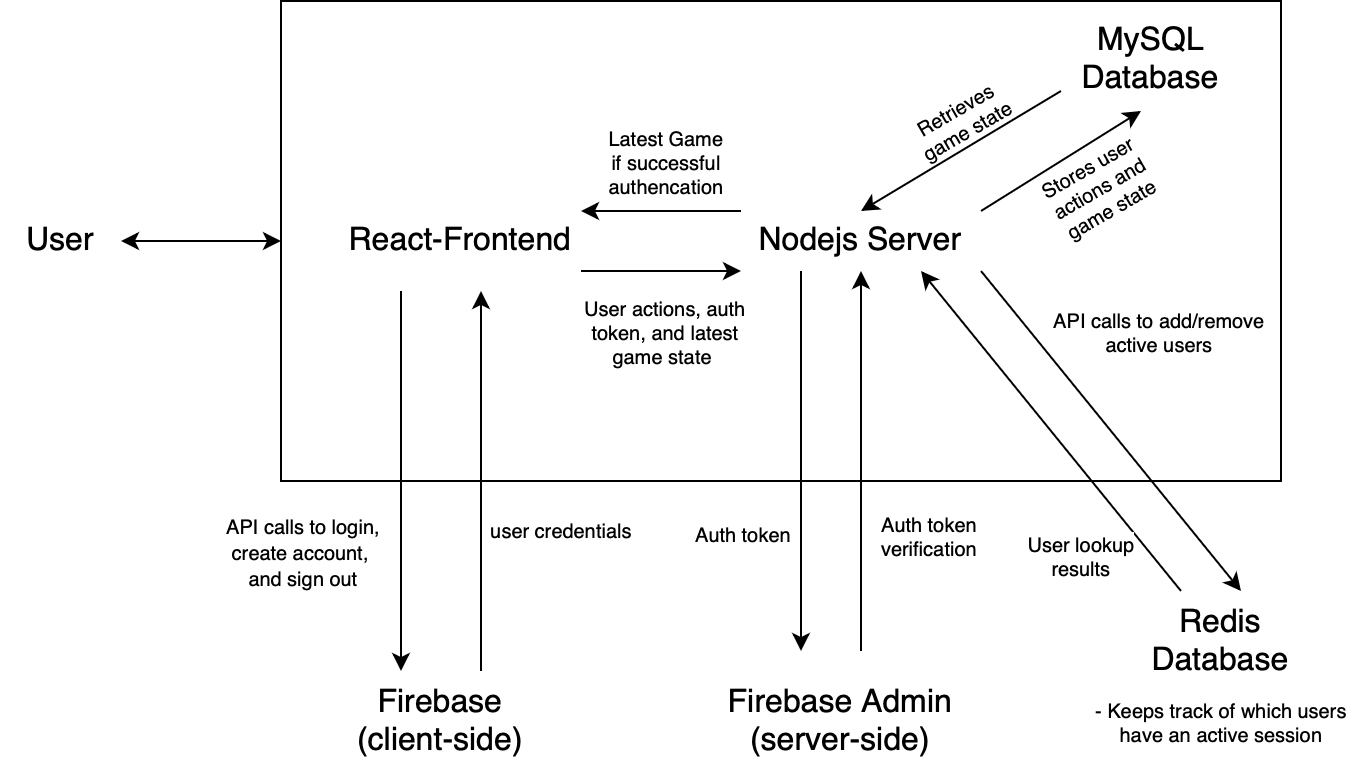
\includegraphics[width=1\textwidth]{SystemBoundary.png}
\caption{System Boundary Diagram}
\label{FigUH}
\end{figure}

\section{Project Overview}

\subsection{Normal Behaviour}

This web game is intended to be played by the participants of the research study. The participants will play on either a desktop computer or laptop with a monitor resolution of at least 1280 by 720, and a stable connection to the internet. This consistency ensures that all research related decisions and relevant game actions are recorded without failure, as to not bias the study.

Normal behaviour of the system includes logging in and out of accounts, buying and selling items, planting and harvesting crop, making research related decisions (i.e whether or not to pay for consulting information or insurance), and ending a turn. Upon ending a turn, all relevant actions are recorded and saved to the database which is used for loading a player's game, and also analyzed as a part of the research.

\subsection{Undesired Event Handling}

Undesired events include users trying to play without any account, users trying to share accounts, users creating bots to play the game, users having an unstable connection to the internet, and users having multiple sessions open.

 To tackle these problems, only authorized users will be able to save their game and have their data tracked. In the case of account sharing, participants within the study will have to understand and accept the guidelines that rule against this. If there is suspicion of account sharing or botting, the account's data will also not be included within the study. If the player loses internet connectivity in between turns, their data would not be able to be uploaded to the database and so to deal with this, the game will resume at the most recently saved state. Lastly, in the undesired case where a user is trying to log into their account in multiple tabs, the system will automatically log them out of the older session to avoid any race conditions.

 
%\wss{How you will approach undesired events}

\subsection{Component Diagram}

\begin{figure}[H]
\centering
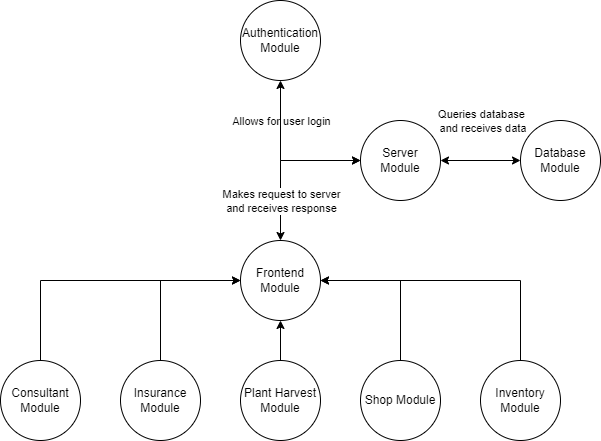
\includegraphics[width=1\textwidth]{component.png}
\caption{Component Diagram for whole system}
\label{FigUH}
\end{figure}

\subsection{Connection Between Requirements and Design} \label{SecConnection}

\begin{enumerate}
    \item \textbf{FR3} To satisfy the requirement of accumulating in game currency, players will be able to sell seeds, items, and harvested crops for money. Players may also gain money from random events.\\
    \item \textbf{FR5, SR1, PR1} To satisfy the requirement of verifying new users as human, users will have to complete a captcha before creating an account.\\
    \item \textbf{FR6} To satisfy the requirement of a shop to purchase items, users will be able to buy seeds, fertilizer, farm buildings, and land.\\
    \item \textbf{FR7} To satisfy the requirement of growing crop, users will be able to plant seeds and fertilizer. Different seeds can be planted on different specific seasons, and they all have their own growth length. Different fertilizer either allow for the harvested crop to be sold for more money than normal, or for the seed to grow faster.\\
    \item \textbf{FR11} To satisfy the requirement of prompting for consulting advice, players will not be able to end their turn unless they respond to the consulting advice prompt. Other NPCs and random events will help disguise this research relevant decisions.\\
    \item \textbf{FR12} To satisfy the requirement of prompting for insurance, players will not be able to end their turn unless they respond to the insurance prompt. Other NPCs and random events will help disguise this research relevant decisions.\\
    \item \textbf{FR13} To satisfy the requirement of logging user decisions, the system will log all game actions that are relevant to the study. These include buying and selling items, and whether or not the player buys consulting advice or insurance.\\
    \item \textbf{FR14} To satisfy the requirement of saving the user's game state, the system will store current money, turn, farm grid, and inventory.\\
    \item \textbf{FR15, LR1} To satisfy the requirement of deleting a user's data, they will have to alert the research conductors and they will remove the user's data from the database.\\
    \item \textbf{FR20} To satisfy the requirement of assigning user's to focus groups, participants will be randomly assigned to either always receive deterministic or probabilistic information from the consultant.\\
    \item \textbf{FR21} To satisfy the requirement of random events, user's will have a chance to be prompted by one after ending their turn. These random events include natural disasters, lucky harvest conditions, and gifts.\\
    \item \textbf{UH1} To satisfy the requirement of being easy to learn, there will be heavy emphasis on using both icons and text for any button.\\
\end{enumerate}

\section{System Variables}
N/A

\section{User Interfaces}
The interface design shown below is the layout of Farming Matters. After the initial phase of development and use, these designs are the most intuitive for navigation and presentation. These designs are open to change during the development and completion of the system. Different colour schemes will also be tested before deciding on a final one. The final user interface will be decided based on the feedback from the developers and initial users. In the designs, all circles will be populated with an appropriate icon.

%\wss{Design of user interface for software and hardware.  Attach an appendix if
%needed. Drawings, Sketches, Figma}

\begin{figure}[H]
\centering
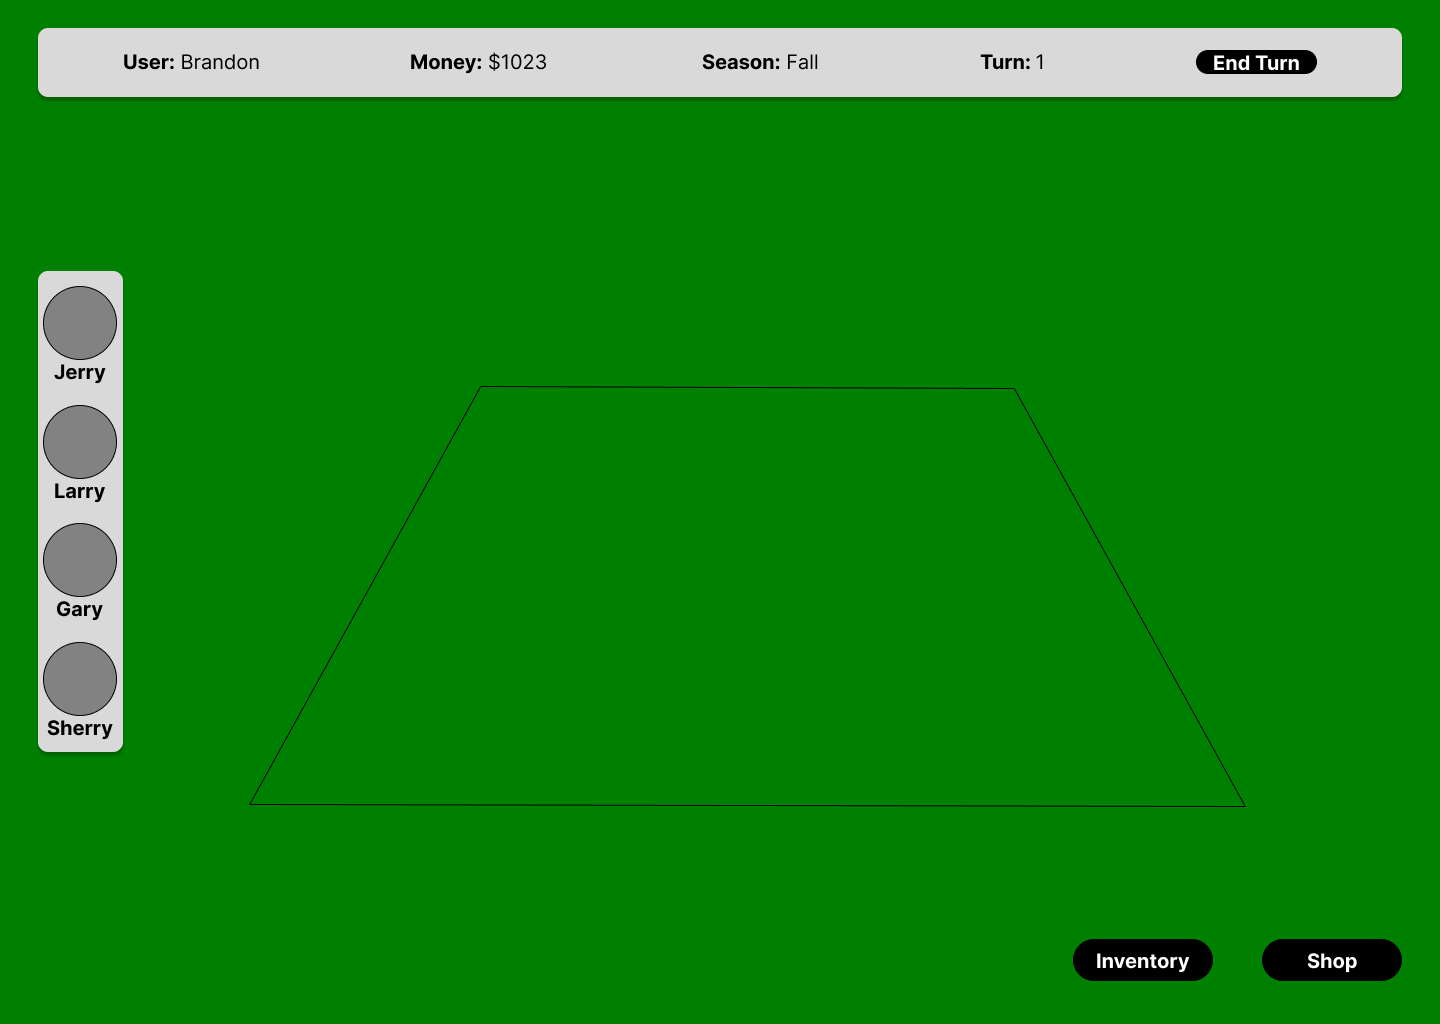
\includegraphics[width=1\textwidth]{main.png}
\caption{Base UI with nothing selected}
\label{FigUH}
\end{figure}

\begin{figure}[H]
\centering
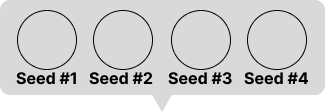
\includegraphics[width=0.5\textwidth]{plant.png}
\caption{Popover for planting a seed}
\label{FigUH}
\end{figure}

\begin{figure}[H]
\centering
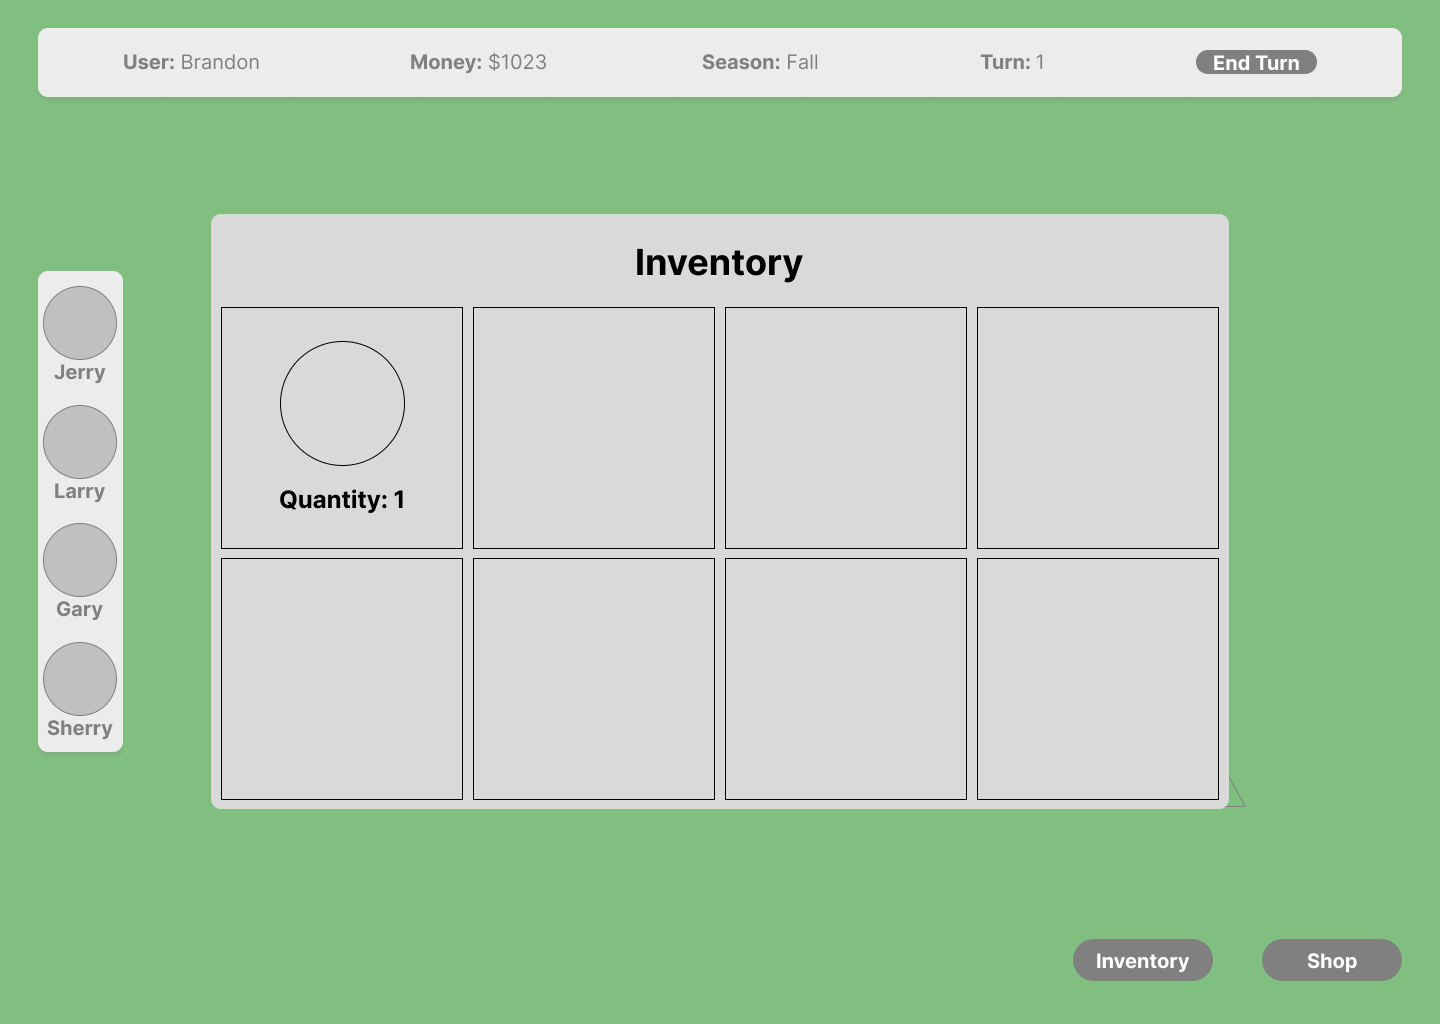
\includegraphics[width=1\textwidth]{inv.png}
\caption{UI for Inventory Screen}
\label{FigUH}
\end{figure}

\begin{figure}[H]
\centering
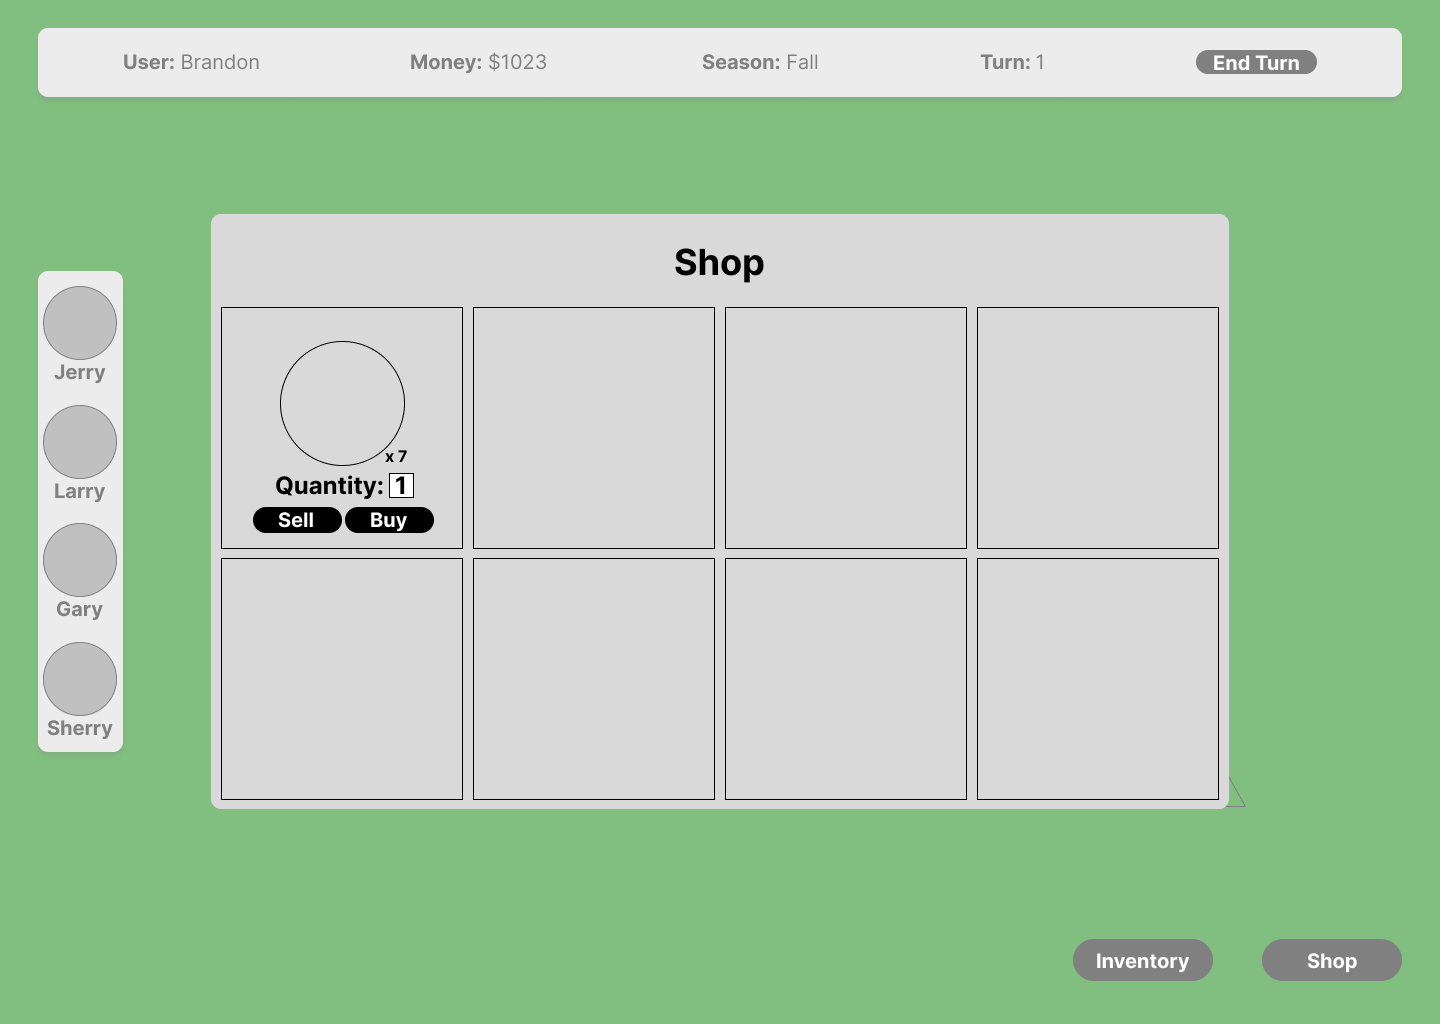
\includegraphics[width=1\textwidth]{shop.png}
\caption{UI for Shop Screen}
\label{FigUH}
\end{figure}

\section{Design of Hardware}
N/A

\section{Design of Electrical Components}
N/A

\section{Design of Communication Protocols}
The system relies on both traditional HTTPS requests and a Websocket connection which persists as long as the user has the application open. HTTPS requests are used to send user actions and game states from client to server, and the server can send the client a saved game state via an HTTPS response. Headers are used in the requests for authorization, so an auth token must be included in any request header. HTTPS is preferred over plain HTTP because the system has login functionality which deals with sensitive data (email/passwords).\\
\\
\\ Websockets are used to track a persistent connection between client and server. Specifically, websockets are leveraged to keep track of each unique user to ensure that a user may not have multiple active sessions. Event handlers on the websocket are used to track the state of the user (logged in or not) and sets the 'active' state of the user respectively. When a client signs out or disconnects, the 'active' state is removed. 

\section{Timeline}

\begin{table}[H]
\centering
\begin{tabular}{p{0.35\textwidth} p{0.3\textwidth}  p{0.3\textwidth}}
\toprule
Module Name & Team Member & Due Date \\
\midrule
Avatar & Andrew & Jan. 1, 2023\\
AvatarMenu & Andrew & Jan. 1, 2023\\
Consultant & Andrew & Jan. 27, 2023\\
OtherAvatar & Andrew & Feb. 3, 2023\\
Item & Mohammad & Jan. 15, 2023\\
Inventory & Mohammad & Jan. 13, 2023\\ 
Market & Mohammad & Jan. 27, 2023\\
DatabaseOperations & Namit & Jan. 29, 2023\\
MusicPlayer & Namit & Feb. 5, 2023\\
GameSettings & Namit & Feb. 10, 2023\\
AuthState & Mihail & Jan. 15, 2023\\
Socket & Mihail & Jan. 20, 2023\\
CilentFirebase & Mihail & Jan. 8, 2023\\
User & Mihail & Jan. 1, 2023\\
AuthError & Mihail & Jan. 1, 2023 \\
CreateAccount & Mihail & Jan. 13, 2023 \\
Login & Mihail & Jan. 13, 2023 \\
ServerFirebase & Mihail, Namit &  Jan. 29, 2023\\
RedisClient & Mihail & Jan. 1, 2023\\
Server & Mihail, Namit, Andrew & Feb. 3, 2023\\
Seed & Brandon & Jan. 20, 2023\\
FarmTile & Brandon & Jan. 27, 2023\\
FarmGrid & Brandon & Dec. 31, 2022\\
GameController & Andrew, Namit, Brandon, Mihail, Mohammad & Feb. 12, 2023 \\
\end{tabular}
\caption{Farming Matters Module Completion Timeline}
\label{TblMH}
\end{table}


% \bibliographystyle {plainnat}
% \bibliography{../../../refs/References}

\newpage{}

\appendix

\section{Interface}
N/A

\section{Mechanical Hardware}
N/A
\section{Electrical Components}
N/A
\section{Communication Protocols}
\begin{itemize}
    \item HTTPS
    \item Websocket
\end{itemize}

\section{Reflection}

The information in this section will be used to evaluate the team members on the
graduate attribute of Problem Analysis and Design.  Please answer the following questions:

\begin{enumerate}
  \item What are the limitations of your solution?  Put another way, given
  unlimited resources, what could you do to make the project better? \\
  
  \smallskip
  The limitations of the solutions include the assets and sound used in the game. The assets were mostly free and given unlimited resources perhaps the look and feel of the project could be improved. Another limitation would be the modularization of the solution. This could be perhaps because of the use of React which supports functional programming better. Another limitation on the solution is the data that can be collected. The ethics board limits us from gathering all data that can be considered unethical and there may be cases where we require certain data but it is not approved. Lastly, the solution has not been thoroughly tested and multiple users need to provide input regarding the solution. With unlimited resources we could gather  more data from a significant number of users.
  \item Give a brief overview of other design solutions you considered.  What
  are the benefits and tradeoffs of those other designs compared with the chosen
  design?  From all the potential options, why did you select documented design?\\
  
  \medskip
  We explored trying to create our own authentication implementation but due to time-constraints and complexity we decided it was better to use Firebase for helping with authentication. Another design that was considered was hosting the MySQL database on the cloud. The main stakeholder rents a server and preferred that the logs were sent to his server and the server would support an SQL database. Some software design considerations the team focused on was deciding where to store the game implementation specific details such that this game logic is kept as a secret from being exploited by users. Intuitively, we considered putting game specific logic in the backend since the user will only have access to client side of the application. However, this will increase the number of requests from the server side to client side, thus putting more stress on the bandwidth and throughput of what the server can handle. Furthermore, causing further delay gameplay wise and hindering the user enjoyment. In the end, we decided to move the game logic to the client side. We have researched and found a way to obfuscation the client side code to prevent others from exploiting the game. 
\\
  
\end{enumerate}

\end{document}